%!TEX root = ../../thesis.tex

\section{Spatial Indexing}
\label{methodology:spatial_index}

Efficient spatial querying is a critical requirement for 3D city model formats, particularly in cloud environments where minimising data transfer is essential. FlatCityBuf implements a packed Hilbert R-tree spatial indexing mechanism \citep{Roussopoulos_Leifker_1985} to enable selective retrieval of city features based on their geographic location. This section details the implementation approach, design decisions, and performance characteristics of the spatial indexing component.

\subsection{Design Attribution}
\label{methodology:spatial_index:attribution}

The spatial indexing mechanism implemented in FlatCityBuf directly adapts the packed Hilbert R-tree approach developed for FlatGeoBuf \citep{horance_2022_detail}. The design combines several key features:

\begin{itemize}
  \item A Hilbert curve-based spatial ordering strategy, inspired by Vladimir Agafonkin's flatbush library, which optimizes data locality for spatially proximate features
  \item A "packed" R-tree implementation, where the tree is maximally filled with no empty internal slots, optimized for static datasets
  \item A bottom-up tree construction methodology that builds the index from pre-sorted features
  \item A flattened tree storage format that enables efficient streaming and remote access
\end{itemize}

The implementation details, including the Hilbert curve encoding algorithm and tree construction process, were sourced from FlatGeoBuf's reference implementation \citep{flatgeobuf_github}. Also, FlatGeoBuf's implementation is also inspired by Vladimir Agafonkin's flatbush library written in JavaScript \citep{vladimir_2018}. The Hilbert curve encoding algorithm, which converts 2D coordinates into a 1D space-filling curve, is based on a non-recursive algorithm described in \citet{hacker_delight_2012}. This approach, known as "2D-C" in spatial indexing literature \citep{hacker_delight_2012}, ensures that features with high spatial locality also have high storage locality, optimizing I/O operations for both local and remote access patterns.

The spatial indexing system is designed to support cloud-native access patterns, allowing efficient retrieval of data directly from cloud storage without requiring a persistent server process. This is achieved through a combination of the Hilbert-sorted feature ordering and the packed R-tree structure, which enables piecemeal access to both the index and feature data over HTTP requests.

It is important to explicitly acknowledge that the spatial indexing code in FlatCityBuf is a direct adaptation of FlatGeoBuf's implementation, with modifications primarily focused on integration with the 3D city model data structure rather than fundamental algorithmic changes. The original implementation by Björn Harrtell and other FlatGeoBuf contributors \citep{flatgeobuf} provided an excellent foundation that has been proven effective for cloud-optimized geospatial data.

While the original FlatGeoBuf implementation targets 2D vector geometries, FlatCityBuf extends this approach to work with 3D city models by using two distinct spatial representations: the 2D bounding box centroid for Hilbert curve ordering, and the full 2D bounding box for spatial intersection tests. This dual representation allows efficient spatial indexing while maintaining accurate spatial query results. The decision to reuse this proven approach rather than developing a novel indexing mechanism was based on FlatGeoBuf's demonstrated effectiveness for cloud-optimized geospatial data formats.

\subsection{Feature sorting}
\label{methodology:spatial_index:feature_sorting}
\todo{add figure here}
A key optimization in FlatCityBuf's indexing strategy is the spatial ordering of features using a Hilbert space-filling curve. This technique enhances data locality by ensuring that features which are spatially proximate in 2D (and 3D) space are also stored close together in the file, thereby optimizing both disk access patterns and HTTP range requests \citep{horance_2022_detail}.

The Hilbert curve encoding process for FlatCityBuf follows these steps:

\begin{enumerate}
  \item For each feature, determine its 2D footprint by calculating the axis-aligned bounding box (minimum and maximum X,Y coordinates) from all vertices across all contained CityObjects
  \item Calculate the geometric centroid of this 2D footprint
  \item Apply a 32-bit Hilbert encoding algorithm to this centroid, converting the 2D spatial position into a 1D ordering value
  \item Sort all features according to their computed Hilbert values in ascending order
  \item During serialization of the sorted features, record both the 2D bounding box and the byte offset (relative position from the start of the feature section) for each feature
\end{enumerate}

These recorded bounding boxes and byte offsets become the foundation for constructing the bottom layer of the R-tree index. The Hilbert encoding implementation uses a non-recursive algorithm described in \citet{hacker_delight_2012}, which has been adapted from the FlatGeoBuf implementation \citep{flatgeobuf_github}, which in turn was inspired by a public domain implementation by \citet{rawrunprotected_2016}.

This approach differs from traditional R-tree construction where nodes are built based on spatial proximity alone. By pre-sorting features along a space-filling curve before constructing the R-tree, FlatCityBuf achieves more predictable and efficient I/O patterns when performing spatial queries \citep{horance_2022_overview}.

\subsection{Index structure}
\label{methodology:spatial_index:index_structure}

The spatial index in FlatCityBuf is implemented as a packed Hilbert R-tree, with a flattened, level-ordered storage structure optimized for efficient traversal over HTTP range requests \citep{horance_2022_detail}. The index is built bottom-up from the sorted features, creating a hierarchical structure where each node represents a spatial region containing its children.

Each index node in the spatial index is represented by a fixed-size binary structure containing:

\begin{itemize}
  \item \textbf{Bounding box coordinates}: 4 little-endian double values (4 bytes each) defining the minimum and maximum X,Y coordinates of the node's bounding box
  \item \textbf{Byte offset}: A 64-byte unsigned integer pointing to either:
    \begin{itemize}
      \item For leaf nodes: The position of the corresponding feature in the features section
      \item For interior nodes: The position of the node's first child in the index section
    \end{itemize}
\end{itemize}

This results in a fixed node size, allowing for predictable memory layouts and efficient search within each node level.

The tree is built using the following process:

\begin{enumerate}
  \item Create the bottom layer (leaf nodes) using the bounding boxes and byte offsets recorded during feature serialization
  \item Group these leaf nodes according to their Hilbert-sorted order into parent nodes, with each parent node containing up to \texttt{index\_node\_size} children (configurable)
  \item Compute the bounding box of each parent node as the union of its children's bounding boxes
  \item Continue building upward, level by level, until a single root node is reached
  \item Serialize the entire tree in level order, starting with the root, then its children, and so on, following the Eytzinger layout pattern (described in \autoref{tb:eytzinger_layout}) to optimise cache line utilization during tree traversal
\end{enumerate}

This "packed" structure ensures that the R-tree is maximally filled (except potentially for the rightmost nodes at each level), which is possible because the tree is built in bulk from a known static dataset. The total size of the index is deterministic and based solely on the number of features and the chosen node size.

Unlike traditional R-trees which support dynamic updates, the packed R-tree in FlatCityBuf is immutable after creation. This trade-off prioritizes read performance and structural efficiency over the ability to modify the dataset, aligning with the file format's primary use case as a cloud-optimized geospatial data delivery mechanism \citep{horance_2022_overview}.

\begin{figure}[ht]
  \centering
  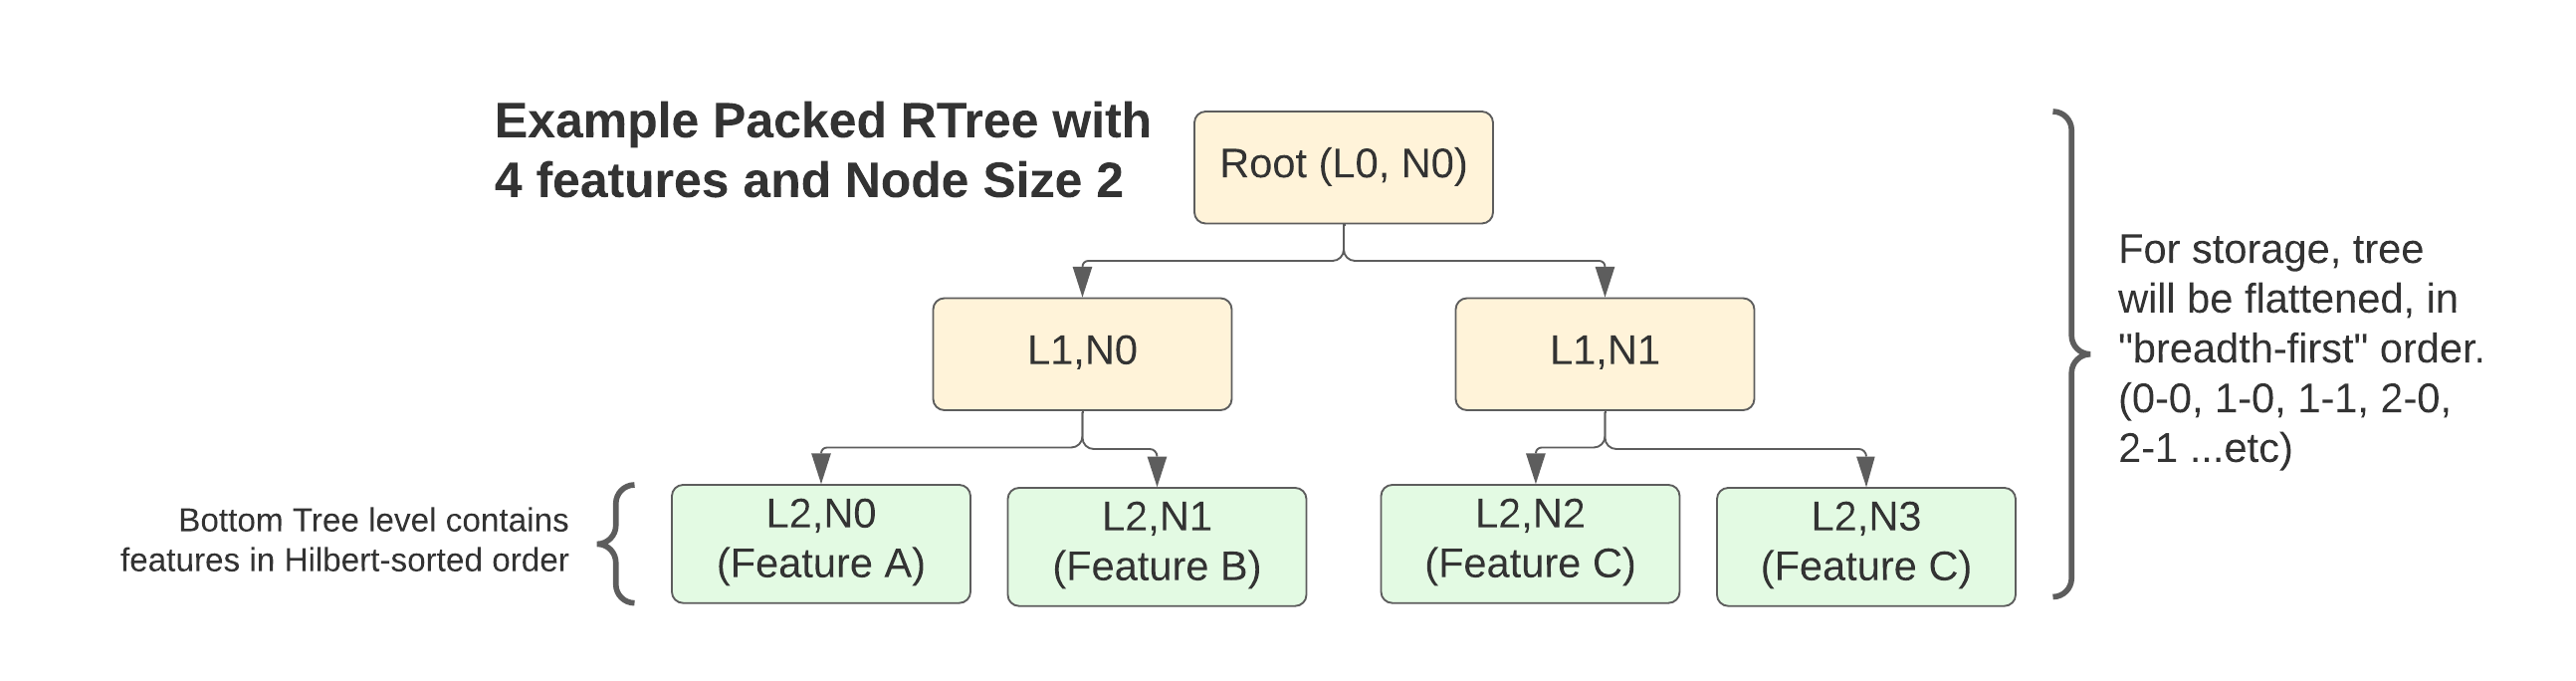
\includegraphics[width=0.9\textwidth]{./figs/methodology/packed_rtree.png}
  \caption{Example of a packed R-tree structure. Image sourced from \cite{horance_2022_overview}.}
  \label{fig:packed_rtree}
\end{figure}
\subsection{2D vs 3D Indexing Considerations}
\label{methodology:spatial_index:2d_vs_3d_indexing}

Although FlatCityBuf is designed for 3D city models, the spatial indexing mechanism deliberately uses a 2D approach rather than a full 3D implementation. This design decision was based on several key observations:

\begin{itemize}
  \item \textbf{Horizontal Distribution}: Most 3D city models are primarily distributed horizontally in global scale, with limited vertical extent relative to their horizontal footprint
  \item \textbf{Query Patterns}: Typical spatial queries for city models focus on horizontal regions (e.g., retrieving buildings within a district), rather than volumetric queries
  \item \textbf{Standards Compatibility}: OGC API - Features - Part 1: Core \citep{ogc_api_2019} and similar standards primarily support 2D spatial querying
  \item \textbf{Implementation Efficiency}: 2D indexing is computationally simpler and more storage-efficient than 3D alternatives
\end{itemize}

Conceptually, the generalization to 3D indexing is possible and would be beneficial for vertically dense metropolitan areas such as Tokyo or New York, where high-rise buildings create vertical distribution of features. In such environments, 3D spatial indexing could improve query performance for volumetric queries that consider height constraints or multi-level urban analysis. However, for the majority of urban environments and current use cases, the 2D approach seems to be sufficient and provides an optimal balance between implementation complexity and query performance.
